\documentclass[dvipdfm]{beamer}
\usepackage{graphicx}

\usepackage{xunicode}
\usepackage{xltxtra}
\XeTeXlinebreaklocale "zh"
\XeTeXlinebreakskip = 0pt plus 1pt
\setsansfont{Vera Sans YuanTi Mono}
\setromanfont{Vera Sans YuanTi Mono}

\usetheme{Madrid} 
%\usecolortheme{seahorse} %sidebartab, rose
\title{基于语义的协作信息检索框架研究}
\author{报告人: 盛艳 \\
导  师: 李云}
\institute{扬州大学信息工程学院}
\date{2009 年 04 月 20 日} 

\begin{document}
\begin{frame}
  \titlepage
\end{frame}

\begin{frame}{概况}
  \tableofcontents
\end{frame}

\section{研究背景及意义}
\begin{frame}[t]{研究背景}
  \begin{block}{}
    \begin{itemize}
    \item 随着因特网的迅猛发展, 网络资源信息迅猛增长. 由于因特网的广泛性和开放性, 在因特网上发布信息极为容易而且不受限制, 无论任何单位, 团体, 个人只要具备上网条件便可以自由地在因特网上发布信息, 从而加剧了因特网信息的急剧膨胀. 如何快速, 准确地从浩瀚的信息资源中寻找所需的信息已经成为困绕用户的一个难题. \pause
    \item 搜索引擎技术要用到信息检索, 人工智能, 计算机网络, 分布式处理, 数据库, 数据挖掘, 数字图书馆, 自然语言处理等多个领域的理论和技术, 所以具有综合性和挑战性. 用户在使用搜索引擎进行信息搜索时, 有时并不十分关注返回结果的多少, 而是看检索结果是否符合自己的需求. 对于一次普通查询, 传统的搜索引擎动辄几十万, 几百万篇文档, 这样的搜索结果是没有多大意义的, 尽管许多搜索引擎利用相关性的技术在这方面做了改进, 但是检索结果相当一部分是用户不感兴趣的, 其主要缺陷就是没有对检索结果筛选和按用户查询意图来组织.
    \end{itemize}
  \end{block}
\end{frame}

\begin{frame}[t]{研究意义}
  \begin{block}{}
    \begin{itemize}
    \item 如何更有意义的表示巨大的信息资源集合? \pause 
    \item 如何对这么多的信息资源进行快速检索? \pause 
    \item 如何更加方便的匹配文档, 找到最具相似性的文档? \pause 
    \item 如何保证检索效率的同时, 返回的结果又是符合用户需要的? 
    \end{itemize}
  \end{block}
\end{frame}

\section{国内外研究现状}
\begin{frame}[t]{国内外研究现状}
  \begin{block}{}
    \begin{itemize}
    \item 在文本分类中, 很多文献提出了不同的方法来特征提取和特征降维, 如利用传统的TF-IDF计算方法, 基于词频差异, 利用CHI公式表示特征对类别的贡献程度和相关程度, 根据特征的类别区分能力进行特征降维, 这些大多从单一角度出发进行特征提取, 使得结果不是很理想, 所以应该统一考虑多种情况. \pause
    \item 国内外针对信息检索领域中提出了很多方法及理论, 如基于布尔模型, 向量空间模型(VSM), 潜在语义索引模型(LSI), 概率模型, 基于统计语言模型的信息检索模型, 基于本体论的信息检索模型等等. 其中, 使用形式概念分析理论来进行信息检索也有很多深入的研究, 使用FCA构建表示信息模型以更确切的表示原始检索模型, 并使用构建出来的概念格进行信息检索, 基于抽象具体程度的不同进行检索可获得独特层面上的检索结果.
    \end{itemize}
  \end{block}
\end{frame}
\begin{frame}[t]{国内外研究现状}
  \begin{block}{}
    \begin{itemize}
    \item 在分布式环境下, 使用FCA理论和技术进行协作信息检索, 这可大大提高检索时间和效率. \pause 
    \item 近年来, 有很多关于个性化和语义检索的工作, 其中, 有相关文献是通过构建用户本体(User Ontology)和一系列语义推理规则进行个性化检索结果返回, 或者使用矢量空间模型和概率模型设计并实现完整的个性化检索系统. 根据用户行为构建的用户描述文件和用户本体(User Ontology)不够准确, 且提取的语义关系也是最基本的, 这导致系统检索效果不是很理想. 又或是在检索过程中 仅基于概率上的规律, 并没有利用关键词间的语义关系和用户历史记录进行分析, 所以很难说检索系统返回的结果就是用户所感兴趣的.
    \end{itemize}
  \end{block}
\end{frame}

\section{论文研究目标}
\begin{frame}[t]{论文研究目标}
  \begin{block}{}
    \begin{itemize}
    \item 针对文本中的\alert{特征提取和约简方法}.\pause
    \item 概念之间的\alert{结构和语义相似度}度量方法.\pause
    \item 协作信息检索系统的分治合并策略.\pause
    \item \alert{用户兴趣模型}的构建方法及\alert{个性化检索模型}. 
    \end{itemize}
  \end{block}
\end{frame}

\section{论文主要内容}
\begin{frame}[t]{论文主要内容}
  \begin{block}{}
    \begin{itemize}
    \item 根据文本各个特征自身和类别信息的统计特性, 提取更少的特征来尽可能的表达出文本蕴含的信息, 得到一种有效的文本特征提取方法, 其中也对文本特征进行约简从而得到少而精的特征信息.\pause
    \item 基于\alert{概念格理论}, 结合\alert{粗糙集理论}和\alert{语义本体理论}, 从形式概念的结构相似和语义相似两个层次上衡量概念间的相似度形式一种有效确切的概念相似度衡量方法.\pause
    \item 针对分布式环境, 提出并构建一个协作信息检索框架, 实现\alert{从结构和语义}两个层次上的概念匹配, 获得更符合用户需求的检索结果.\pause
    \item 在对检索结果排序过程中, 利用\alert{语义本体WordNet}对用户历史检索记录进行分析, 从而构建用户兴趣模型, 以便更精确的表达出用户兴趣所在, 并按照此模型对初始检索结果重新排序.
    \end{itemize}
  \end{block}
\end{frame}

\section{采取的研究方案及可行性分析}
\begin{frame}[t]{采取的研究方案及可行性分析}
  \begin{block}{基于类别分析及有效特征提取的文本分类方法}
    \begin{itemize}
    \item 结合人类语言中普遍存在的\alert{Zipf定律}, 对大量文本集进行全局的特征提取. $$ P(r)=\frac{C}{r^\alpha}$$ \pause 
    %\centering 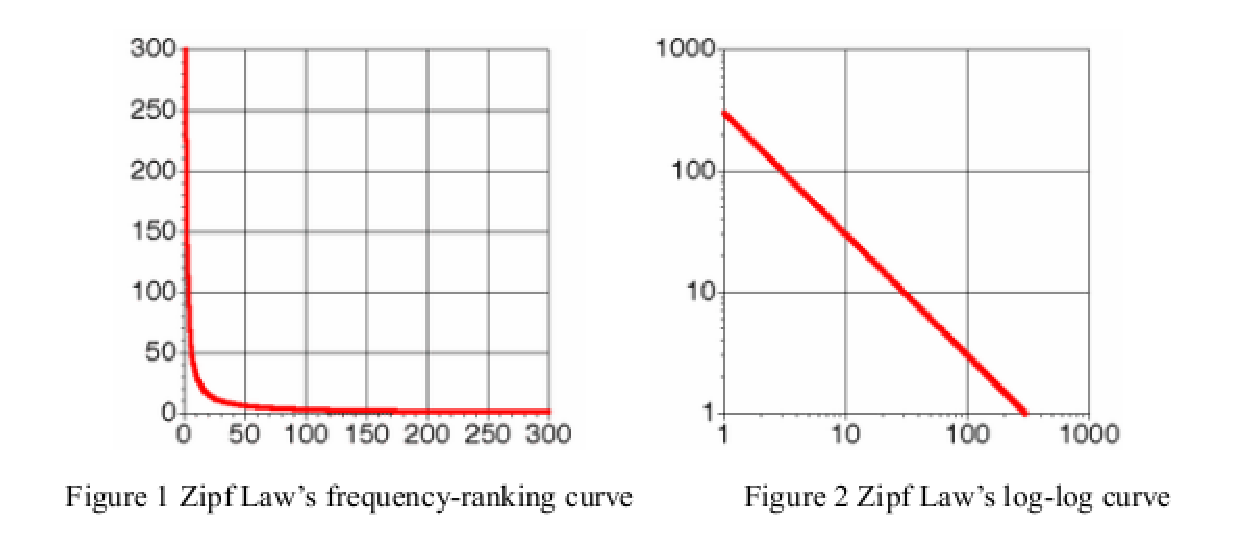
\includegraphics[height=4cm]{zipf.eps}
    \item 在计算每个特征词的类别频率CF之后, 对文本集进行类内局部特征提取. \\ \small{CF计算公式: $$ CF(t, C_i)=\frac{the\; times\; of\; t\; appears\; in\; c_i}{the\; number\; of\; all\; words\; in\; c_i} $$ }
    \end{itemize}
  \end{block}
\end{frame}

\begin{frame}[t]{采取的研究方案及可行性分析}
  \begin{block}{基于类别分析及有效特征提取的文本分类方法}
    \begin{itemize}
    \item 在CF基础上, 提出一个特征权值公式. \small{$$ \omega(t,d)=\frac{TF(t,d)\times\log(IDF(t)+\sigma)\times max_{c \in C}CF(t,c)}{\sqrt{\sum_{t \in d}(TF(t,d)\times\log(IDF(t)+\sigma)\times max_{c \in C}CF(t,c))^2}}$$ } \pause
    \item 最后, 使用提出的权值公式, 改进K近邻算法, 对标准数据集NewsGroup进行文本自动分类测试, 得到效果如下图:
    \end{itemize}
  \end{block}
\end{frame}

\begin{frame}[t]{采取的研究方案及可行性分析}

    \centering 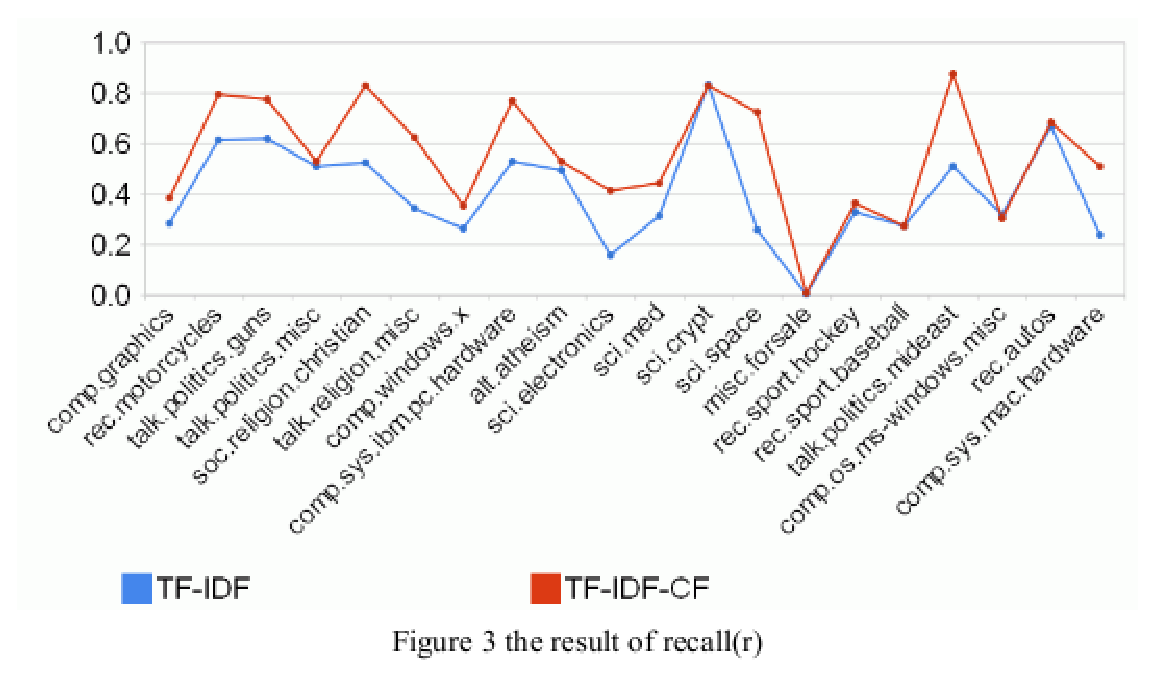
\includegraphics[height=3cm]{category1.eps}
    \centering 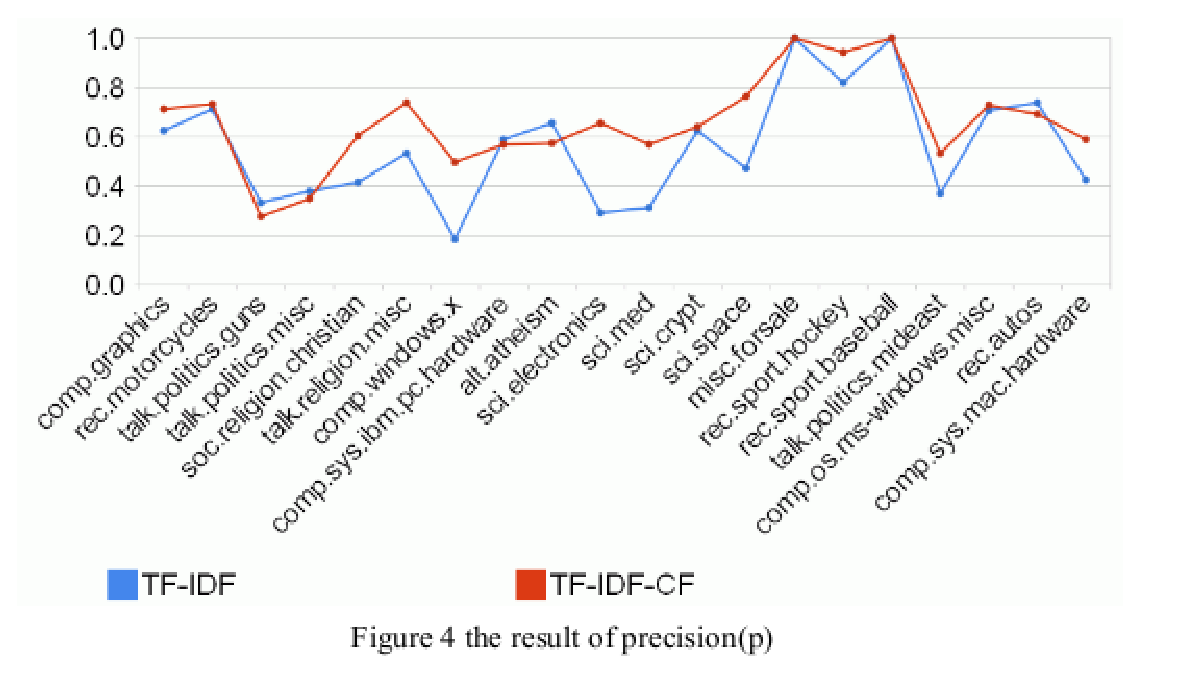
\includegraphics[height=3cm]{category2.eps} \\
    \centering 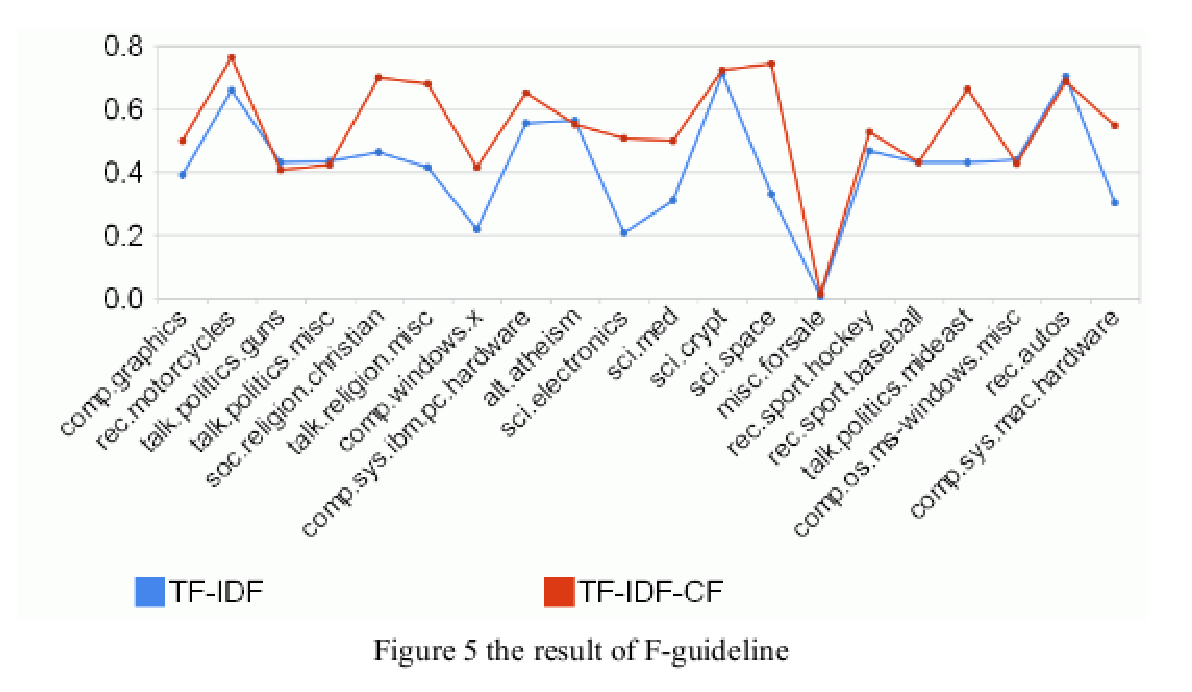
\includegraphics[height=3cm]{category3.eps}

\end{frame}

\begin{frame}[t]{采取的研究方案及可行性分析}
  \begin{block}{结构及语义层次上的概念相似度衡量方法}
    \begin{itemize}
    \item 针对文本特征的形式背景, 按照已经成熟的概念格构造算法, 使用粗糙集中的下近似并结合概念的层次信息, 语义本体的语义信息衡量概念间的相似度.\pause
    \item 结构相似度计算方法 \tiny{$$ StructSim(C_1,C_2)=\frac{\lvert (B_1 \cap B_2)_{LA} \rvert}{\lvert (B_1 \cup B_2)_{LA} \rvert+\alpha(C_1, C_2)\lvert B_{1LA} - B_{2LA} \rvert+(1-\alpha(C_1, C_2))\lvert B_{2LA} - B_{1LA} \rvert} $$ }\pause
    \item \small{语义相似度的计算是通过Wordnet找到词之间的相互关系, 通过一定策略进行量化. $$ SemanticSim(C_1,C_2)=\frac{M(B_1, B_2)}{max\{\lvert B_1\rvert, \lvert B_2\rvert\}}$$ }
    \end{itemize}
  \end{block}
\end{frame}

\begin{frame}[t]{采取的研究方案及可行性分析}
  \begin{block}{一种基于WordNet的检索结果个性化排序方法}
    \begin{itemize}
    \item 在对检索结果排序过程中, 利用\alert{语义本体WordNet}对用户历史检索记录进行分析, 从而构建用户兴趣模型, 以便更精确的表达出用户兴趣所在, 并按照此模型对初始检索结果重新排序. 此用户模型是通过寻找各个历史关键词之间的联系进行构建, 最终构建的如下图所示:  \\
    \centering 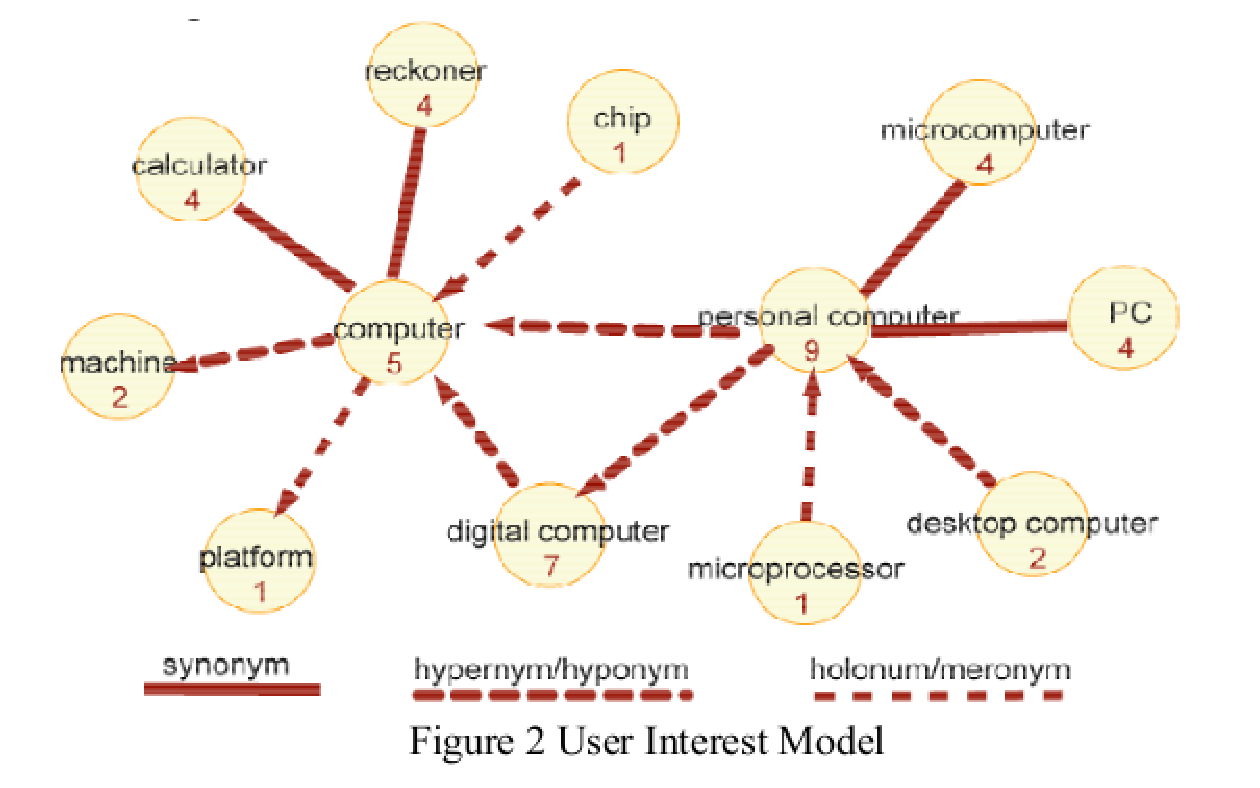
\includegraphics[height=4cm]{uim.eps}
    \end{itemize}
  \end{block}
\end{frame}

\section{论文技术路线}
\begin{frame}[t]{论文技术路线}
  \begin{block}{基于FCA的协作信息检索框架}
    \begin{itemize}
    \item 分布式环境下, 采用先分后合策略, 对多个独立的形式概念格进行概念匹配后合并为最终结果返回给用户.\pause 整体框图如下所示: 
    \centering 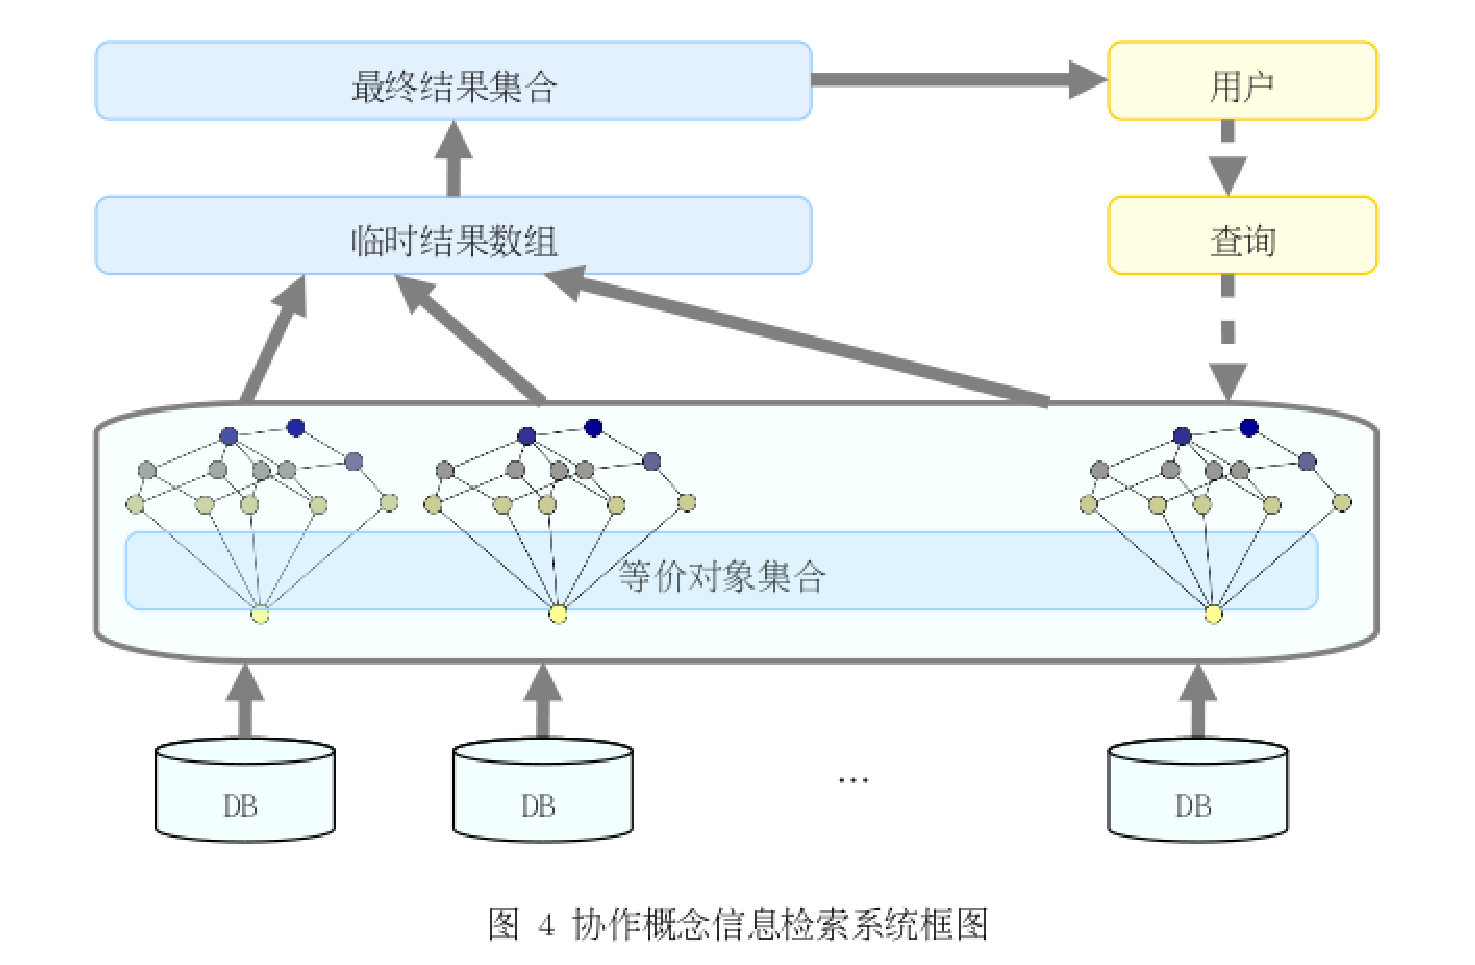
\includegraphics[height=5.6cm]{fcair.eps}
    \end{itemize}
  \end{block}
\end{frame}

\begin{frame}[t]{论文技术路线}
  \begin{block}{总结}
    \begin{itemize}
    \item 用具体实例验证所提模型, 方法和算法.
    \item \alert{FCA}, \alert{文本特征提取策略}, \alert{语义本体}, \alert{粗糙集}的理论提供了思想, 方法和算法的研究基础.
    \end{itemize}
  \end{block}
\end{frame}

\section{论文后续扩展}
\begin{frame}[t]{论文后续扩展}
  \begin{block}{应用方向}
    \begin{itemize}
    \item 协作信息检索性能提高
    \item 利用本体的用户兴趣模型更新及维护
    \item 扩展到中文领域 
    \end{itemize}
  \end{block}
  \begin{block}{理论方向}
    \begin{itemize}
    \item  语义相似的进一步研究
    \end{itemize}
  \end{block}
\end{frame}

\begin{frame}[t]{}
  \begin{block}{参与的科研项目与发表论文}
    \begin{itemize}
    \item \small{面向本体的形式概念分析扩展模型及算法(60575035), 国家自然科学基金项目}
    \item \small{序列概念格扩展模型及其序列模式挖掘算法研究(08KJB520012), 江苏省教育厅高校自然科学研究计划项目}
    \item \small{基于概念格模型的本体构建与运算, 扬州大学信息工程学院研究生创新基金项目}
    \item \small{一种基于概念格的本体合并方法, 微电子学与计算机, Vol.25, NO.9, 2008:34-36}
    \item \small{基于概念格模型的本体映射, 南京师范大学学报(工程技术版), Vol.8, NO.4, 2008:91-94, 获第三届江苏计算机大会(JSCC2008)优秀论文}
    \item \small{A Rough Concept Lattice Model of Variable Precision, Proc. of IITA 2008 :162-166}
    \item \small{A Text Classification Method with an Effective Feature Extraction based on Category Analysis(已投)}
    \item \small{A Personalized Search Results Ranking Method Based on WordNet (已投)}
    \end{itemize}
  \end{block}
\end{frame}

\begin{frame}{}
\begin{center}\huge{谢谢大家!}\end{center}
\end{frame}

\end{document} 
